\documentclass[landscape]{article}
\usepackage[utf8]{inputenc}
\usepackage[T1]{fontenc}

\usepackage[margin=1in]{geometry}
\usepackage{tikz-qtree}
\usetikzlibrary{shadows,trees}
\begin{document}
\tikzset{font=\small,
edge from parent fork down,
level distance=1.75cm,
every node/.style=
    {top color=white,
    bottom color=blue!25,
    rectangle,rounded corners,
    minimum height=8mm,
    draw=blue!75,
    very thick,
    drop shadow,
    align=center,
    text depth = 0pt
    },
edge from parent/.style=
    {draw=blue!50,
    thick
    }}

\centering
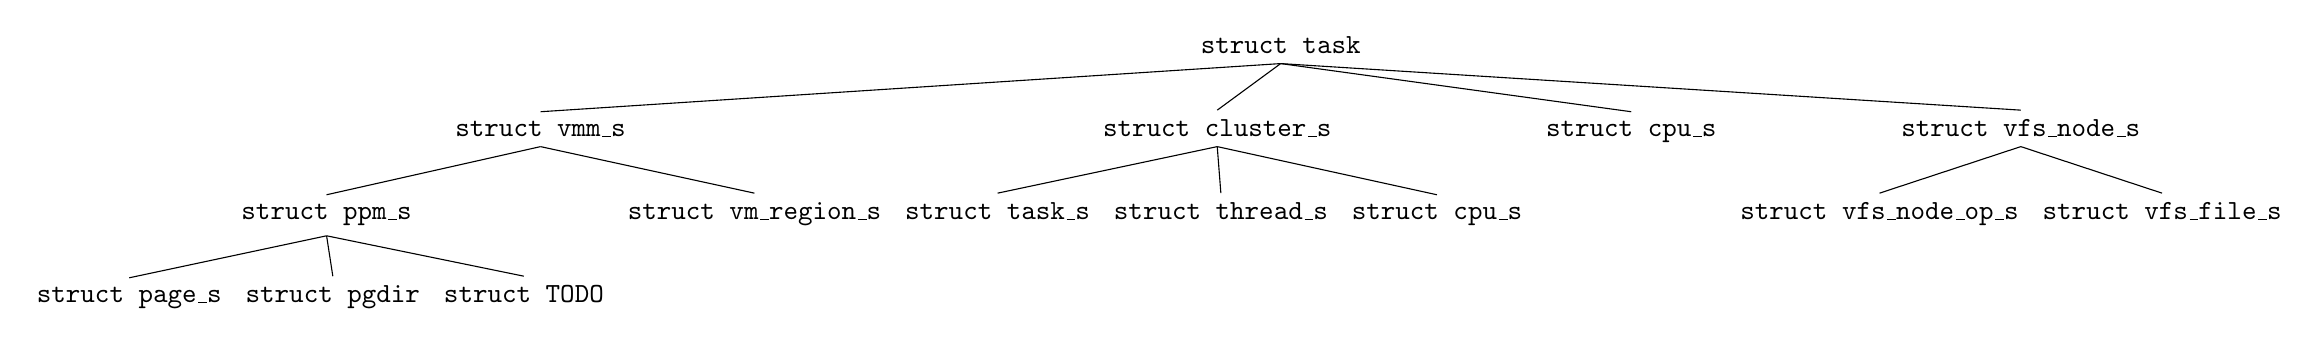
\begin{tikzpicture}
\Tree [.\texttt{struct task}
        [.{\texttt{struct vmm\_s}}
            [.{\texttt{struct ppm\_s}}
              [.{\texttt{struct page\_s}} ]
              [.{\texttt{struct pgdir}} ]
              [.{\texttt{struct TODO}} ] ]
            [.{\texttt{struct vm\_region\_s}} ] ] 
        [.{\texttt{struct cluster\_s}}
            [.{\texttt{struct task\_s}} ]  
            [.{\texttt{struct thread\_s}} ]
            [.{\texttt{struct cpu\_s}} ] ]
        [.{\texttt{struct cpu\_s}} ]
        [.{\texttt{struct vfs\_node\_s}}
            [.{\texttt{struct vfs\_node\_op\_s}} ]
            [.{\texttt{struct vfs\_file\_s}} ] ]
]
\end{tikzpicture}
\end{document}
